\chapter{Fundamentação teórica}
\label{cap:fundamentacao}

\section{A malha do MPAS-A: tesselação de Voronoi centroidal esférica}

A malha horizontal do \mpasa{} é uma \emph{tesselação de Voronoi
centroidal esférica} (\textit{Spherical Centroidal Voronoi Tessellation},
SCVT) \cite{skamarock2012voronoi, dugunzburger2002cvt, yang2017cvtsphere}.
Dado um conjunto de pontos geradores $\{\mathbf{x}_i\}_{i=1}^{N}$
distribuídos sobre a esfera, o diagrama de Voronoi particiona a
superfície em $N$ células $\{V_i\}$, onde cada célula é o lugar
geométrico dos pontos da esfera mais próximos do gerador $\mathbf{x}_i$
do que de qualquer outro gerador:
\begin{equation}
  V_i = \left\{ \mathbf{x} \in \mathbb{S}^2 \;:\; d(\mathbf{x}, \mathbf{x}_i) \le d(\mathbf{x}, \mathbf{x}_j) \ \forall j \ne i \right\},
  \label{eq:voronoi_def}
\end{equation}
com $d(\cdot,\cdot)$ a distância geodésica sobre a esfera. A tesselação é
dita \emph{centroidal} quando cada gerador $\mathbf{x}_i$ coincide com o
centroide (baricentro de massa) de sua própria célula $V_i$ -- uma
condição de otimalidade obtida iterativamente pelo algoritmo de Lloyd, e
que produz células com forma próxima de hexágonos regulares na maior
parte do domínio, minimizando distorção de área e permitindo refinamento
local suave da resolução horizontal sem as descontinuidades abruptas de
grades aninhadas tradicionais.

No \mpasa{}, as variáveis prognósticas de massa (densidade seca $\rho$,
temperatura potencial $\theta$, razões de mistura de água $q$) são
armazenadas nos centros de célula $\mathbf{x}_i$ (geradores da
tesselação), enquanto a componente \emph{normal} do vento horizontal $u$
é armazenada nas arestas entre células vizinhas -- um posicionamento tipo
\emph{C-grid} (Arakawa C) generalizado para malha não estruturada. Essa
convenção de estagiamento é o que motiva a separação, na interpolação
horizontal nativa apresentada neste trabalho (\cref{cap:fase1}), entre um
tratamento para campos de massa (posicionados no centro da célula) e um
tratamento posterior, distinto, para a reconstrução do vento nas arestas
(\cref{cap:fase3}).

\section{Dualidade com a triangulação de Delaunay}
\label{sec:dualidade}

Toda tesselação de Voronoi possui uma estrutura geométrica \emph{dual}: a
\emph{triangulação de Delaunay}, obtida conectando por um segmento (ou,
na esfera, um arco geodésico) cada par de geradores cujas células de
Voronoi compartilham uma aresta. A propriedade central dessa dualidade,
usada diretamente neste trabalho, é que os \emph{vértices} da malha de
Voronoi (pontos onde três ou mais células se encontram) são exatamente os
\emph{circuncentros} dos triângulos da triangulação de Delaunay --
enquanto os \emph{centros das células} de Voronoi (os geradores
$\mathbf{x}_i$) são exatamente os \emph{vértices} dos triângulos de
Delaunay.

\begin{figure}[H]
  \centering
  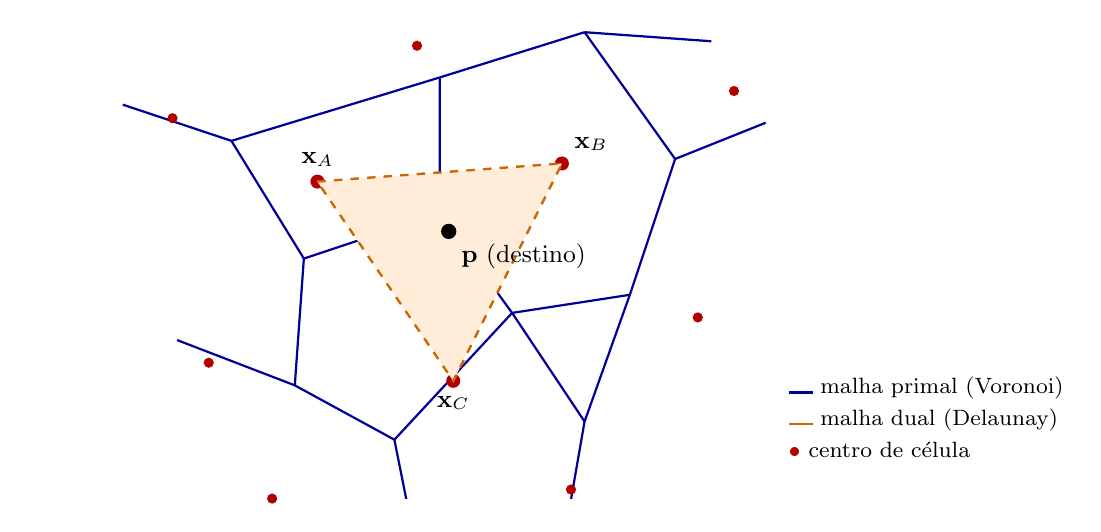
\begin{tikzpicture}[scale=1.15, every node/.style={font=\small}]
    % --- celulas de Voronoi (poligonos irregulares esquematicos) ---
    \begin{scope}
      \clip (-4.6,-2.6) rectangle (4.6,2.6);
      % geradores (centros de celula)
      \coordinate (A) at (-1.4, 0.9);
      \coordinate (B) at ( 1.3, 1.1);
      \coordinate (C) at ( 0.1,-1.3);
      \coordinate (D) at (-2.6,-1.1);
      \coordinate (E) at ( 2.8,-0.6);
      \coordinate (F) at (-0.3, 2.4);
      \coordinate (G) at (-3.0, 1.6);
      \coordinate (Hp) at ( 3.2, 1.9);
      \coordinate (I) at ( 1.4,-2.5);
      \coordinate (J) at (-1.9,-2.6);

      % arestas de Voronoi (esquematicas, desenhadas a mao para ilustrar hexagonos)
      \draw[thick, blue!60!black]
        (-0.05,2.05) -- (1.55,2.55)
        (1.55,2.55) -- (2.55,1.15)
        (2.55,1.15) -- (2.05,-0.35)
        (2.05,-0.35) -- (0.75,-0.55)
        (0.75,-0.55) -- (-0.05,0.55)
        (-0.05,0.55) -- (-0.05,2.05);
      \draw[thick, blue!60!black]
        (-0.05,0.55) -- (-1.55,0.05)
        (-1.55,0.05) -- (-1.65,-1.35)
        (-1.65,-1.35) -- (-0.55,-1.95)
        (-0.55,-1.95) -- (0.75,-0.55);
      \draw[thick, blue!60!black]
        (-1.55,0.05) -- (-2.35, 1.35)
        (-2.35,1.35) -- (-0.05,2.05);
      \draw[thick, blue!60!black]
        (0.75,-0.55) -- (1.55,-1.75)
        (1.55,-1.75) -- (2.05,-0.35);
      \draw[thick, blue!60!black]
        (-1.65,-1.35) -- (-2.95,-0.85);
      \draw[thick, blue!60!black]
        (-0.55,-1.95) -- (-0.35,-2.95);
      \draw[thick, blue!60!black]
        (1.55,-1.75) -- (1.35,-2.9);
      \draw[thick, blue!60!black]
        (1.55,2.55) -- (2.95,2.45);
      \draw[thick, blue!60!black]
        (2.55,1.15) -- (3.55,1.55);
      \draw[thick, blue!60!black]
        (-2.35,1.35) -- (-3.55,1.75);
    \end{scope}

    % --- geradores / centros de celula ---
    \foreach \p/\lbl in {A/$\mathbf{x}_A$, B/$\mathbf{x}_B$, C/$\mathbf{x}_C$}
      \fill[red!70!black] (\p) circle (2.2pt);
    \foreach \p in {D,E,F,G,Hp,I,J}
      \fill[red!70!black] (\p) circle (1.6pt);

    % --- triangulo dual de Delaunay em torno do ponto de interesse ---
    \coordinate (P) at (0.05, 0.35);
    \draw[thick, dashed, orange!80!black] (A) -- (B) -- (C) -- cycle;
    \fill[orange!15] (A) -- (B) -- (C) -- cycle;
    \draw[thick, dashed, orange!80!black] (A) -- (B) -- (C) -- cycle;

    % ponto de interesse (ex.: centro de celula da malha de DESTINO)
    \fill[black] (P) circle (2.4pt);
    \node[below right=1pt] at (P) {$\mathbf{p}$ (destino)};

    \node[above=2pt] at (A) {$\mathbf{x}_A$};
    \node[above right=1pt] at (B) {$\mathbf{x}_B$};
    \node[below=2pt] at (C) {$\mathbf{x}_C$};

    \node[align=left, anchor=west, font=\footnotesize] at (3.7,-1.7)
      {\textcolor{blue!60!black}{\rule{1em}{1pt}} malha primal (Voronoi)\\[2pt]
       \textcolor{orange!80!black}{\rule{1em}{1pt}} malha dual (Delaunay)\\[2pt]
       \textcolor{red!70!black}{\textbullet} centro de célula};
  \end{tikzpicture}
  \caption{Esquema da dualidade Voronoi--Delaunay usada na interpolação
    horizontal nativa. As células poligonais (azul) formam a malha
    primal de Voronoi; conectando os centros de três células mutuamente
    vizinhas obtém-se um triângulo do dual de Delaunay (laranja). Um
    ponto arbitrário $\mathbf{p}$ -- tipicamente o centro de célula da
    malha de \emph{destino} -- é localizado dentro de um único triângulo
    de Delaunay da malha de \emph{origem}, e o campo escalar nesse ponto
    é obtido por interpolação baricêntrica dos três valores nos vértices
    do triângulo (\cref{eq:baricentrica}).}
  \label{fig:voronoi_delaunay}
\end{figure}

\section{Interpolação baricêntrica no triângulo dual}
\label{sec:baricentrica}

Dado um triângulo de Delaunay com vértices $\mathbf{x}_A, \mathbf{x}_B,
\mathbf{x}_C$ (centros de três células de Voronoi mutuamente vizinhas) e
um ponto de interesse $\mathbf{p}$ localizado dentro desse triângulo, as
\emph{coordenadas baricêntricas} $(\lambda_A, \lambda_B, \lambda_C)$ de
$\mathbf{p}$ são os únicos pesos que satisfazem simultaneamente
\begin{equation}
  \mathbf{p} = \lambda_A \mathbf{x}_A + \lambda_B \mathbf{x}_B + \lambda_C \mathbf{x}_C,
  \qquad
  \lambda_A + \lambda_B + \lambda_C = 1,
  \qquad \lambda_A, \lambda_B, \lambda_C \ge 0.
  \label{eq:baricentrica_def}
\end{equation}
Geometricamente, cada peso $\lambda_A$ é proporcional à área do
subtriângulo oposto ao vértice $A$ (formado por $\mathbf{p}$, $B$ e $C$),
normalizada pela área total do triângulo $ABC$:
\begin{equation}
  \lambda_A = \frac{\text{Área}(\mathbf{p}, B, C)}{\text{Área}(A,B,C)},
  \qquad
  \lambda_B = \frac{\text{Área}(A, \mathbf{p}, C)}{\text{Área}(A,B,C)},
  \qquad
  \lambda_C = \frac{\text{Área}(A, B, \mathbf{p})}{\text{Área}(A,B,C)}.
  \label{eq:baricentrica_area}
\end{equation}
O valor interpolado de um campo escalar $\phi$ (por exemplo, temperatura,
altura geopotencial, ou umidade específica) no ponto $\mathbf{p}$ é então
a combinação linear
\begin{equation}
  \phi(\mathbf{p}) \approx \lambda_A\, \phi(\mathbf{x}_A) + \lambda_B\, \phi(\mathbf{x}_B) + \lambda_C\, \phi(\mathbf{x}_C).
  \label{eq:baricentrica}
\end{equation}
Esse método é exato para campos que variam linearmente sobre o triângulo
e, criticamente para este trabalho, é \emph{exato por construção} quando
o ponto de interesse $\mathbf{p}$ coincide com um dos próprios vértices
$\mathbf{x}_A$, $\mathbf{x}_B$ ou $\mathbf{x}_C$ (nesse caso um dos pesos
vale $1$ e os outros dois valem $0$) -- é essa propriedade que permite
validar a implementação de forma direta: interpolando o campo de uma
malha para si mesma (\emph{auto-\emph{scatter}}), o erro deve ser
identicamente nulo em todas as células (\cref{sec:validacao_fase1}).

Na esfera, o procedimento operacional usado pelo motor de pesos (herdado
sem modificação do utilitário \texttt{convert\_mpas} da NCAR, ver
\cref{sec:fase1_reuso}) é: (i)~localizar, para cada ponto de destino
$\mathbf{p}$, o triângulo de Delaunay da malha de origem que o contém,
usando a conectividade célula-célula/aresta já armazenada na malha
(\texttt{cellsOnCell}, \texttt{cellsOnVertex}); (ii)~calcular os três
pesos baricêntricos via \cref{eq:baricentrica_area}, com as áreas
computadas sobre a superfície esférica; e (iii)~aplicar
\cref{eq:baricentrica} a cada campo escalar requisitado. A reconstrução
do vento, por armazenar sua componente normal nas arestas em vez de um
vetor completo no centro de célula, exige um tratamento adicional --
descrito em detalhe na \cref{sec:vento_arestas} -- baseado em Funções de
Base Radial (RBF) para reconstrução vetorial nos centros de célula,
seguida de projeção na direção normal de cada aresta de destino.

\section{Coordenada vertical \textit{terrain-following} híbrida}
\label{sec:coord_vertical_teoria}

Na direção vertical, o \mpasa{} usa uma coordenada $\zeta$
\emph{terrain-following} (segue o relevo perto da superfície e tende a
superfícies de altura constante longe dele), na formulação híbrida de
Klemp \cite{klemp2011terrainfollowing}. A altura física $z$ de uma
superfície de coordenada constante $\zeta=\zeta_k$ é dada por
\begin{equation}
  z(\zeta_k, \mathbf{x}) = \zeta_k + A(\zeta_k)\, h_s(\mathbf{x}, \zeta_k),
  \label{eq:coord_hibrida_teoria}
\end{equation}
onde $h_s$ é uma versão \emph{suavizada} do terreno (progressivamente
mais suave em níveis mais altos, para atenuar erros de gradiente de
pressão horizontal sobre relevo íngreme -- o problema clássico que
motivou toda a família de coordenadas híbridas desde Gal-Chen e
Simmons/Burridge até Klemp) e $A(\zeta)$ é uma função de atenuação que
vale $1$ na superfície e decai suavemente a $0$ numa altura de transição
$z_t$, definindo o ponto acima do qual as superfícies de coordenada
voltam a ser perfeitamente horizontais. As formas específicas de
$A(\zeta)$ e do algoritmo de suavização de $h_s$ efetivamente usadas pelo
\mpasa{} -- e reproduzidas neste trabalho -- são detalhadas com suas
constantes exatas no \cref{cap:fase2}.

\section{Balanço hidrostático de referência}
\label{sec:hidrostatico_teoria}

A condição inicial de um modelo não hidrostático como o \mpasa{} ainda
precisa de um estado \emph{base} hidrostaticamente balanceado, em torno
do qual as variáveis prognósticas são definidas como perturbações. O
\mpasa{} usa uma atmosfera de referência isotérmica seca
($T_0=\SI{250}{\kelvin}$), e o campo de pressão real é obtido resolvendo
iterativamente a relação hidrostática discreta na direção vertical --
não uma integração fechada, mas um esquema numérico que usa exatamente
os mesmos coeficientes de interpolação vertical ($f_{zm}$, $f_{zp}$) já
definidos pela grade vertical da \cref{sec:coord_vertical_teoria}, de
modo que o campo de massa final seja consistente, ponto a ponto, com a
métrica vertical adotada. O algoritmo completo, incluindo a formulação
não trivial de densidade seca acoplada à métrica vertical
($\rho_{zz}=\rho/\partial z/\partial \zeta$), está detalhado no
\cref{cap:fase4}.
